\documentclass[10pt,twocolumn]{article}
\usepackage{graphicx}
\graphicspath{{./Figures/}}
\usepackage[margin=0.5in]{geometry}
\usepackage[cmex10]{amsmath}
\usepackage{array}
\usepackage{booktabs}
\usepackage{mathtools}
\title{\textbf{Optimization Assignment - 2}}
\author{Bole Manideep}
\date{September 2022}

\providecommand{\brak}[1]{\ensuremath{\left(#1\right)}}

\begin{document}

\maketitle
\paragraph{\textit{Problem Statement} - Find the maximum and minimum values, if any, of the function given by \\ $f(x) = -\brak{x-1}^2+10$.} 

\section*{\large Solution}
Generally,
\begin{align*}
\brak{x-1}^2 \geq 0 \hspace{5mm} \forall \hspace{1mm} x \in \mathbf{R} \\
\implies -\brak{x-1}^2 \le 0 \\
\implies -\brak{x-1}^2+10 \le 10 \\
\implies f(x) \le 10
\end{align*}
Therefore, $f(x)$ has a maxima and the maximum value of the function is 10.



\section*{\large Gradient Ascent Method}
\begin{align*}
x_{n+1} &= x_n + \alpha \nabla f(x_n) \\
\implies x_{n+1} &= x_n + \alpha \nabla f(-\brak{x_n-1}^2+10)
\end{align*}
Taking $x_0 = 1, \alpha = 0.001$ and $precision = 0.00000001$, values obtained using python are:
\begin{align}
\boxed{\text{Maxima} = 10.0} \\
\boxed{\text{Maxima Point} = 1.0}
\end{align}

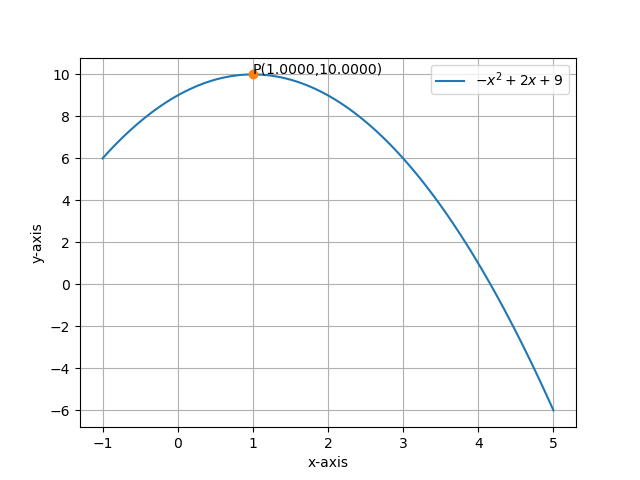
\includegraphics[width=1\columnwidth]{opt2.png}
\centering \text{Graph of f(x) = $-\brak{x-1}^2+10$}

\end{document}
